
\begin{figure}
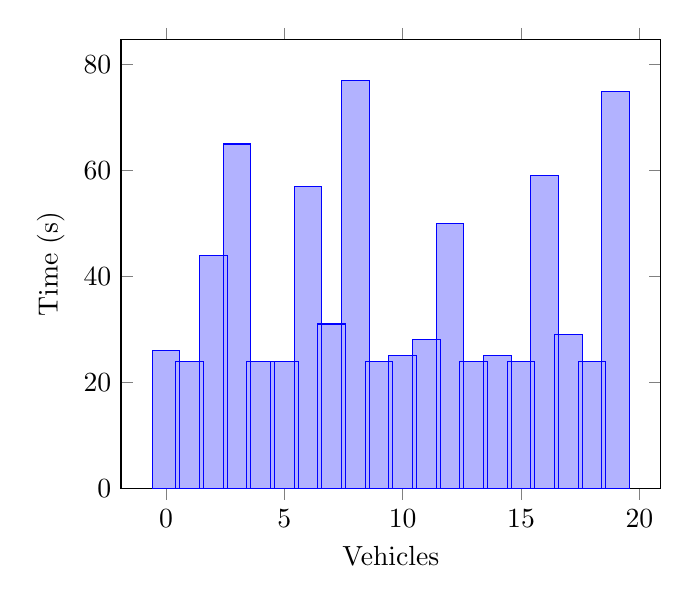
\begin{tikzpicture}
\begin{axis}[
legend style={anchor=west},
xlabel=Vehicles,
ylabel=Time (s),
ymin=0,
ybar,
]
\addplot coordinates {
(0, 26)
(1, 24)
(2, 44)
(3, 65)
(4, 24)
(5, 24)
(6, 57)
(7, 31)
(8, 77)
(9, 24)
(10, 25)
(11, 28)
(12, 50)
(13, 24)
(14, 25)
(15, 24)
(16, 59)
(17, 29)
(18, 24)
(19, 75)
};

\end{axis}
\end{tikzpicture}
\label{tik:100:2_O, 2_O.-60, 1_N}
\caption{100 percent diving with GSC on route $2_O, 2_O.-60, 1_N$}
\end{figure}
